\documentclass[%
	%draft
	]{ijsra}
\def\IJSRAidentifier{\currfilebase} %<---- don’t change this!
%-------Title | Email | Keywords | Abstract-------------
\def\maintitle{Quantification of Interpersonal Violence in Skeletal Remains from Medieval and Post-Medieval London}
\def\shorttitle{Interpersonal Violence in Skeletal Remains from London}
\def\cmail{dannicroucher1@gmail.com }
\def\keywords{violence, trauma, medieval, post-medieval, London, gender and biological sex}
%\def\keywordname{}%<--- redefine the name “Keywords“ in needed language
\def\abstract{With little published work on the subject of gender targeting in violence from archaeological skeletal remains, this paper explores the knowledge vacuum by analysing data from interpersonal violence markings, resultant of purposeful violence between two or more people, on skeletal remains to determine how rates of skeletal trauma differ over time between the sexes. This quantitative study utilises data from the Museum of London Archaeology’s (MOLA) osteological WORD database from the medieval period, dating AD 1050-1540, and post-medieval period, 16th to 19th centuries (WORD Database 2016). Despite well-established trends through numerous studies outlining the decline in violence from the medieval period to modern society, the data reveals the rate of interpersonal violence increased against males by \SI{35}{\percent} from the medieval period to the post-medieval period, whilst the rate declined against females by \SI{13.3}{\percent}. 
The rise in male violence is suggested to be a consequence of war injuries, continued post-war raids on London, economic stress, or sample size limitations. Furthermore the data indicates that violence was rarely received peri-mortem for either sex, suggesting trauma was seldom fatal despite its predominate location on the crania. Finally, the findings suggest violence was predominantly perpetrated through blunt and sharp force mechanisms and that violence became less widespread and accepted by the post-medieval period in London, as the number of sites within which individuals with interpersonal violence were found decreased across the periods. This conclusion is supported by historic evidence from courts of laws outlining public disapproval of violence perpetrated against females and outlawing lethal violence (Gurr 1981).}
%--------Author’s names------------
\def\authorone{Dannielle Croucher}
%-------Biographical information-------------
\def\bioone{Dannielle is an Exeter University graduate, with a first class honours degree in Bsc Archaeology and Forensic Science. Dannielle graduated from Exeter with the Lady Aileen Fox award for the leading dissertation in the department, from which this publication is based. She went on to present this work in oral presentations at Oxford University’s graduate conference (GAO) and UCL’s Society of Archaeological Masters conference (SAMS), alongside poster presentations at the UK Archaeological Science conference (UKAS) and the Forensic Archaeology, Anthropology and Ecology Symposium (FAAE) across 2016 and 2017. 
At the time of publication, Dannielle was completing an Msc in Bioarchaeology and Forensic Anthropology at University College London, which she is predicted to finish in September 2017 with a distinction. After September, Dannielle aims to work as a research assistant before commencing a PhD in osteology, researching gender bias and body mass within forensic and archaeological contexts.}
%------University/Institution--------------
\def\affilone{University College London (UCL)}

\begin{filecontents}{\IJSRAidentifier.bib}
%Bibliography-data HERE

@BOOK {allmand1988,
    author    = "Allmand, C.",
    title     = "The Hundred Years War: England and France at War c. 1300-c. 1450",
    publisher = "Cambridge University Press",
    year      = "1988"
}
@ARTICLE {anderson2002,
    author  = "Anderson, C. and Bushman, B.",
    title   = "Human Aggression",
    journal = "Annual Review of Psychology",
    year    = "2002",
    volume  = "53",
    pages   = "27-51"
}
@BOOK {baker1992,
    author    = "Baker, S. and O’Neill, B. and Ginsburg, M. and Li, G.",
    title     = "The Injury Fact Book",
    publisher = "New York: Oxford University Press",
    year      = "1992",
    edition   = "Second"
}
@ARTICLE {beattie1974,
    author  = "Beattie, M.",
    title   = "The Pattern of Crime in England, 1660-1800",
    journal = "Past and Present",
    year    = "1974",
    volume  = "62",
    pages   = "47-95"
}
@BOOK {belknap2001,
    author    = "Belknap, J.",
    title     = "The Invisible Woman: Gender, Crime and Justice",
    publisher = "Belmont, CA: Wadsworth",
    year      = "2001"
}
@ARTICLE {berger1995,
    author  = "Berger, T. and Trinkaus, E.",
    title   = "Patterns of trauma among Neanderthals.",
    journal = "Journal of Archaeological Science",
    year    = "1995",
    volume  = "2",
    pages   = "841-852"
}
@BOOK {brownstein2000,
    author    = "Brownstein, H.",
    title     = "Social Reality of Violence and Violent Crime",
    publisher = "Prentice Hall",
    year      = "2000"
}
@ARTICLE {buikstra1994,
    author  = "Buikstra, J. and Ubelaker, D.",
    title   = "Standards for Data Collecting from Human Skeletal Remains",
    journal = "Fayeteville, Arkansas: Arkansas Archaeological Survey Report Number 44",
    year    = "1994"
}
@ARTICLE {burda2007,
    author  = "Burda, M. and Hamermesh, D and Weil, P.",
    title   = "Total Work, Gender and Social Norms",
    journal = "The National Bureau of Economic Research",
    year    = "2007",
    number  = "13000"
}
@BOOK {byers2002,
    author    = "Byers, S.",
    title     = "Introduction to Forensic Anthropology: a Textbook",
    publisher = "Boston: Auyn and Bacon",
    year      = "2002"
}
@BOOK {cockburn1977,
    author    = "Cockburn, J.",
    title     = "The Nature and Incidence of Crime in England, 1559-1625: A Preliminary Survey in Crime in England 1550-1800",
    publisher = "Princeton University Press",
    year      = "1977"
}
@ARTICLE {deaux1985,
    author  = "Deaux, K.",
    title   = "Sex and Gender",
    journal = "Annual Review of Psychology",
    year    = "1985",
    volume  = "36",
    pages   = "60-61"
}
@ARTICLE {dewees2003,
    author  = "DeWees, M. and Parker, K.",
    title   = "Women, Region, and Types of Homicide",
    journal = "Homicide Studies.",
    year    = "2003",
    volume  = "7",
    number  = "4",
    pages   = "368-393"
}
@ARTICLE {eisner2001,
    author  = "Eisner, M.",
    title   = "Modernization, Self-Control and Lethal Violence. The Long-Term Dynamics of European Homicide Rates",
    journal = "British Journal of Criminology",
    year    = "2001",
    volume  = "41",
    pages   = "618-638."
}
@ARTICLE {eisner2003,
    author  = "Eisner, M.",
    title   = "Long-Term Historical Trends in Violent Crime",
    journal = "Crime and Justice.",
    year    = "2003",
    volume  = "30",
    pages   = "83-142"
}
@BOOK {elias1976,
    author    = "Elias, N",
    title     = "The Civilizing Process",
    publisher = "Oxford University Press",
    year      = "1976",
    volume    = "1-2"
}
@BOOK {fox1994,
    author    = "Fox, J.",
    title     = "Uniform Crime Reports of the United States: Supplementary Homicide Report, 1976-1992",
    publisher = "Boston, MA: Northeastern University College of Criminal Justice",
    year      = "1994"
}
@BOOK {frayer1997,
    author    = "Frayer, D.",
    title     = "Ofnet: Evidence for a Mesolithic massacre. In: Martin, D. Frayer, D. Troubled Times: Violence and Warfare in the Past",
    publisher = "Gordon and Breach",
    year      = "1997"
}
@BOOK {freestone2012,
    author    = "Freestone, S",
    title     = "The Pestilence of London: Women, Hygiene, Prostitution and Pollution",
    publisher = "University of Chicago, NEPCA",
    year      = "2012",
    volume    = "49"
}
@BOOK {galloway1999,
    author    = "Galloway, A.",
    title     = "Broken bones. Anthropological analysis of blunt force trauma",
    publisher = "Charles C Thomas",
    year      = "1999"
}
@ARTICLE {gardiner2001,
    author  = "Gardiner, J.",
    title   = "An analysis of the pathology of the Krapina Neanderthals",
    journal = "American Journal of Physical Anthropology",
    year    = "2001",
    volume  = "35"
}
@BOOK {given1977,
    author    = "Given, B.",
    title     = "Society and State Homicide in Thirteenth-Century England",
    publisher = "Stanford University Press",
    year      = "1977"
}
@BOOK {goldstein2003,
    author    = "Goldstein, J.",
    title     = "War and Gender: How Gender Shapes the War System and Vice Versa",
    publisher = "Cambridge University Press",
    year      = "2003"
}
@BOOK {goodman1990,
    author    = "Goodman, A.",
    title     = "The Wars of the Roses: military activity and English society, 1452-97",
    publisher = "Taylor \& Francis",
    year      = "1990"
}
@ARTICLE {gurr1981,
    author  = "Gurr, T.",
    title   = "Historical Trends in Violent Crime: A Critical Review of the Evidence",
    journal = "Crime and Justice",
    year    = "1981",
    volume  = "3",
    pages   = "295-353"
}
@ARTICLE {hendricks2007,
    author  = "Hendricks, S. Jenkins, E and Anderson, K.",
    title   = "Trends in workplace homicides in the U.S, 1993–2002: A decade of decline",
    journal = "American Journal of Industrial Medicine",
    year    = "2007",
    volume  = "50",
    number  = "4",
    pages   = "316–325."
}
@ARTICLE {krahn1986,
    author  = "Krahn, H. Hartnagel, T. and Gartrell, J.",
    title   = "Income Inequality and Homicide Rates: Corss-National Data and Criminological Theories",
    journal = "Criminology",
    year    = "1986",
    volume  = "24",
    number  = "2",
    pages   = "269"
}
@BOOK {lorber1994,
    author    = "Lorber, J.",
    title     = "Paradoxes of Gender",
    publisher = "Vail-Ballou Press",
    year      = "1994"
}
@ARTICLE {lovell1997,
    author  = "Lovell, N.",
    title   = "Trauma Analysis in Paleopathology",
    journal = "Yearbook of Physical Anthropology",
    year    = "1997",
    volume  = "40",
    pages   = "139-170"
}
@ARTICLE {mackinnon1982,
    author  = "MacKinnon, C.",
    year = "1982",
    title   = "Feminism, Marxism, Method, and the State: An Agenda for Theory",
    journal = "Feminist Theory",
    volume  = "7",
    number  = "3",
    pages   = "515-544"
}
@BOOK {martin1998,
    author    = "Martin, D. and Frayer, D.",
    year = "1998",
    title     = "Troubled Times: Violence and Warfare in the Past",
    publisher = "Gordon and Breach"
}
@ARTICLE {mccall2008,
    author  = "McCall, G. and Shields, N.",
    title   = "Examining the evidence from small-scale societies and early prehistory and implications for modern theories of aggression and violence",
    journal = "Aggression and Violent Behaviour",
    year    = "2008",
    volume  = "13",
    pages   = "1-9"
}
@ARTICLE {mccullough2008,
    author  = "McCullough, A.",
    title   = "Female Gladiators in Imperial Rome: Literary Context and Historical Fact",
    journal = "Classical World",
    year    = "2008",
    volume  = "101",
    number  = "2",
    pages   = "197-209"
}
@ARTICLE {mercy1989,
    author  = "Mercy, J. and Saltzman, L.",
    title   = "Fatal violence among spouses in the United States, 1976-85",
    journal = "American Journal of Public Health",
    year    = "1989",
    volume  = "79",
    number  = "5",
    pages   = "595-599"
}
@BOOK {meyerson2004,
    author    = "Meyerson. M, Thiery, D. and Falk, O.",
    title     = "A Great Effusion of Blood?: Interpreting Medieval Violence",
    publisher = "University of Toronto Press",
    year      = "2004"
}
@BOOK {moore1997,
    author    = "Moore, J and Scott, E.",
    title     = "Invisible people and processes: Writing gender and childhood into European archaeology",
    publisher = "Leicester University",
    year      = "1997"
}
@ARTICLE {pohl1998,
    author  = "Pohl, J.",
    title   = "Themes of Drunkenness, Violence, and Factionalism in Tlaxcalan Altar Paintings",
    journal = "Anthropology and Aesthetics",
    year    = "1998",
    volume  = "33",
    number  = "184-207."
}
@TECHREPORT {rand1997,
    author      = "Rand, M.",
    title       = "Violence-Related Injuries Treated in Hospital Emergency Departments",
    institution = "Bureau of Justice Statistics Special Report; U.S. Department of Justice",
    year        = "1997",
    number      = "NCJ-156921."
}
@ARTICLE {redfern2009,
    author  = "Redfern, R.",
    title   = "Does Cranial Trauma Provide Evidence for Projectile Weaponry in Late Iron Age Dorset?",
    journal = "Oxford Journal of Archaeology",
    year    = "2009",
    volume  = "28",
    number  = "4",
    pages   = "399-424."
}
@BOOK {redfern2008,
    author    = "Redfern, R.",
    title     = "A bioarchaeological analysis of violence in Iron Age females: a perspective from Dorset, England. In:. Changing Perspectives on the First Millennium B.C.",
    publisher = "Oxbow Books",
    year      = "2008"
}
@ARTICLE {redfern2011,
    author  = "Redfern, R.",
    title   = "A Re-appraisal of the Evidence for Violence in the Late Iron Age Human Remain from Maiden Castle Hillfort, Dorset, England",
    journal = "Proceedings of the Prehistoric Society",
    year    = "2011",
    volume  = "77",
    pages   = "111-138."
}
@BOOK {redfern2013,
    author    = "Redfern, R.",
    title     = "A Bioarchaeological analysis of violence in Iron Age females: Dorset, England. 4th c BC- 1st c AD. In: The Archaeology of Violence",
    publisher = "State University of New York Press.",
    year      = "2013"
}
@ARTICLE {redfern2014,
    author  = "Redfern, R. and Bonney, H.",
    title   = "Headhunting and amphitheatre combat in Roman London, England: new evidence from the Walbrook Valley",
    journal = "Journal of Archaeological Sciences",
    year    = "2014"
}
@ARTICLE {richards2000,
    author  = "Richards, M. and Pettitt, P. and Trinkaus, E. and Smith, F. and Paunovic, M. and Karavanic, I.",
    title   = "Neanderthal diet at Vindija and Neanderthal predation: The evidence from stable isotopes",
    journal = "PNAS",
    year    = "2000",
    volume  = "97"
}
@ARTICLE {robb1997,
    author  = "Robb, J.",
    title   = "Violence and gender in early Italy. In: Troubled Times. Violence, warfare in the past",
    journal = "War and Society",
    year    = "1997",
    volume  = "3",
    pages   = "111-144"
}
@BOOK {roberts2003,
    author    = "Roberts, C. and Cox, M.",
    title     = "Health and disease in Britain from Prehistory to the Present Day",
    publisher = "Sutton Publishing Ltd.",
    year      = "2003"
}
@ARTICLE {rodwel1997,
    author  = "Rodwel, M. and Byers, K.",
    title   = "Auditing Constructivist Inquiry: Perspectives of Two Stakeholders",
    journal = "Qualitative Inquiry",
    year    = "1997",
    volume  = "3",
    number  = "1",
    pages   = "116-134"
}
@ARTICLE {saltmarsh1941,
    author  = "Saltmarsh, J.",
    title   = "Plague and Economic Decline in England in The Later Middle Ages",
    journal = "Cambridge Historical Journal",
    year    = "1941",
    volume  = "7",
    pages   = "23-41."
}
@BOOK {samaha1974,
    author    = "Samaha, J.",
    title     = "Law and Order in Historical Perspective: The Case of Elizabethan Essex",
    publisher = "Academic Press",
    year      = "1974"
}
@ARTICLE {sharpe1985,
    author  = "Sharpe, J.",
    title   = "The History of Violence in England: Some Observations",
    journal = "Past and Present",
    year    = "1985",
    volume  = "108",
    pages   = "206–15"
}
@ARTICLE {stone1983,
    author  = "Stone, L.",
    title   = "Interpersonal Violence in English Society 1300–1980",
    journal = "Past and Present",
    year    = "1983",
    volume  = "101",
    number  = "1",
    pages   = "22-33."
}
@BOOK {turvey2010,
    author    = "Turvey, R.",
    title     = "The Wars of the Roses and Henry VIII: Britain 1450-1509",
    publisher = "Hodder Education",
    year      = "2010"
}
@ARTICLE {udry1994,
    author  = "Udry, R.",
    title   = "The nature of gender",
    journal = "Demography",
    year    = "1994",
    volume  = "31",
    number  = "4",
    pages   = "561-573."
}
@ARTICLE {unger1979,
    author  = "Unger, R.",
    title   = "Towards the redefinition of sex and gender",
    journal = "American Psychologist",
    year    = "1979",
    volume  = "34",
    number  = "11",
    pages   = "1085-1094"
}
@BOOK {walker1997,
    author    = "Walker, P.",
    title     = "Wife beating, boxing and broken noses: skeletal evidence for the cultural patterning of interpersonal violence. In: Troubled Times: Violence and Warfare in the Past",
    publisher = "Gordon \& Breach",
    year      = "1997"
}
@ARTICLE {walker2001,
    author  = "Walker, P.",
    title   = "A Bioarchaeological Perspective on the History of Violence",
    journal = "Annual Review of Anthropology",
    year    = "2001",
    volume  = "30",
    pages   = "573-590."
}
@ONLINE {museumoflondoncentreforbioarchaeologymedieval,
    author = "Museum of London Centre for Bioarchaeology",
    title  = "Medieval Data",
    url    = "http://archive.museumoflondon.org.uk/Centre-for-Human-Bioarchaeology/Resources/Medievaldatadownloads.htm"
}
@ONLINE {museumoflondoncentreforbioarchaeologypostmedieval,
    author = "Museum of London Centre for Bioarchaeology",
    title  = "Post-Medieval Data",
    url    = "http://archive.museumoflondon.org.uk/Centre-for-Human-Bioarchaeology/Resources/Post-medievaldatadownloads.htm"
}
@TECHREPORT {worldhealthorganization2002,
    author      = "World Health Organization",
    title       = "World Report on Violence and Health: Summary",
    institution = "World Health Organization",
    year        = "2002"
}
@BOOK {wrangham1996,
    author    = "Wrangham, R. and Peterson, D",
    title     = "Demonic males: Apes and the evolution of human violence",
    publisher = "Houghton Mifflin",
    year      = "1996"
}



\end{filecontents}
\IJSRAopening%<---- don’t change this!
%-------

% \IJSRAseparator


\IJSRAsection{Research Aims}
\lettrine{T}{his} research was conducted to elucidate how interpersonal violence trauma trends changed between males and females through the quantification of the numeracy of violent markings present on the skeletal remains of individuals from medieval and post-medieval London. The research explores how  violence levels are connected to social climate and how it differs between the sexes, through the quantification of ‘normative violence rates’, defined as violent interactions occurring due to social and cultural cues, excluding external causes such as war \parencites{brownstein2000}{meyerson2004}. The number of injuries sustained from each violent encounter and the injury mechanism, understood by the type of trauma sustained, were noted and compared, allowing for a comparison between the number of fractures, projectile injuries and blunt and sharp force traumas between the time periods. Location of trauma was also analysed, alongside comparing the numbers of anti- and peri-mortem traumas. 

\IJSRAsection{Research Context}

The significance of violence can be understood when viewed in modern context; it is a leading cause of death for 15-44 year olds and 1.4 million people in the U.S. received medical treatment for interpersonal violence in 1994 alone \parencites{rand1997}{redfern2013}{worldhealthorganization2002}. Violence is explained as a universal condition by 
\textcite{mccall2008}, occurring in different forms across the world: verbally, passively and physically, with no civilisation void of its incidence 
\parencites{baker1992}{lovell1997}. Physical interpersonal violence, defined as injury between two individuals caused intentionally through extrinsic force, 
can be explored archaeologically through the direct evidence of violence preserved on skeletal remains, confirming the occurrence of aggression \parencites{lovell1997}{klein1999}{gardiner1999}{walker2001}. 

Equally present across society is the concept of ‘gender’. Anthropologically and biologically, the concepts of gender and biological sex are clearly defined; the former being a social and cultural construct and the latter a biological absolute \parencites{unger1979}{deaux1985}[385]{white2005}. Moreover, the well-defined social definitions of gender undeniably dictate treatment of males and females, with violence following these sculpted concepts \parencites{gurr1981}{belknap2001}{mccall2008}. 
Whilst skeletal remains are analysed to determine biological sex, sex does not necessarily conform to modern gender ideas, with gender equating to different psychological definitions across different time periods, locations and cultures, and because within each society “being [male or] female varies according to culture and social experience” \parencite{redfern2013}. 
Subsequently, modern ideals of violence may not conform to historical actualities.  Preconceived ideas of the transitional role of males and females from the medieval to the post-medieval period often suggest females to progressively develop a more domestic and less physical role within society, whilst males maintained an active role \parencite{robb1997}.  
The association of lower levels of violence with higher domestication would suggest females to have consequently experienced lower levels of aggressive interactions in the post-medieval period. It has equally been proposed that violence levels decreased uniformly with time as both males and females became increasingly civilised with progressing social and economic advancements, however these analyses failed to use skeletal evidence to quantify trauma \parencite{beattie1974}.  

The intertwining of gender and violence can be demonstrated through the analysis of violence within modern society \parencite{hendricks2007}. 
Statistical analyses of homicide, strangulation, stabbing, firearm injuries and beatings suggest both perpetrators and victims of modern violence to be predominantly young males \parencite{baker1992}.  
Analyses further indicate a 10:1 male to female perpetration ratio in modern America \parencite{anderson2002} and stated \SI{65.2}{\percent} 
of homicides to be male-male in 2004, U.S. (U.S. Bureau of Statistics 2006). Equally, males accounted for three-fifths of victims treated for violence in hospital emergency departments in a study of American hospitals (1990). 

Female perpetration of interpersonal violence, however, has been poorly researched, a consequence of low data availability as only 10-29\% of homicides in the US are perpetrated by females \parencite{dewees2003}. 
However, research shows females are at higher risk of becoming victims of domestic, community and state violence \parencite{worldhealthorganization2002}. 
This knowledge vacuum is mirrored historically as past sources predominantly depict violence as male dominated, typically including warfare, knighthood and gladiator practises \parencites{pohl1998}{mccullough2008}. 
The ‘gender’ bias has fuelled research into the role of biological sex in violence within cultures, enlightening complexities within gender margins across time and societies \parencite{moore1997}. 
Social research has formed theorems ranging from the Marxist approach, analysing limitations of biological physique differences between the sexes, to contrasting gender-dominated theories in patriarchal and feminist schools of thought \parencites{mackinnon1982}{lorber1994}{udry1994}{burda2007}. 
‘Gender’ however, has not been extensively archaeologically explored through skeletal trauma analysis to determine the role of both sexes within violence in pre-modern societies \parencites{krahn1986}{martin1998}{belknap2001}.

Within archaeology skeletal remains are the “only independent and direct evidence of violence and aggression” \parencite[1]{redfern2013}.  
Consequently, analysis of preserved violent markings on skeletal remains facilitates understanding of pre-modern violence victimisation without bias \parencite{robb1997}. 
Sociobiological evolutionary theories exploring the history of violence predict that ancestral violence patterns reflect modern aggression levels.  Models suggest violence to have maintained a high prevalence as females were more likely to mate with males who violently out-competed other males, leading to stronger, more aggressive offspring, attempting to explain the exclusion of females within violence \parencites{wrangham1996}{mccall2008}. 

Pre-historically, interpersonal violence can be seen on hominid skeletons from Africa, Asia and Europe dating to the Middle Pleistocene \parencite{klein1999}. 
The \textcite{berger1995} study of 200 Neanderthals from Europe and the Near East indicated high frequencies of cranial, neck, and torso trauma in comparison to hospital populations from New York and London. Five of the Neanderthal skeletons exhibiting cranial and neck trauma were male, with only one possible female present. 
Contrastingly, the earliest evidence of mass murder effecting 38 Middle Paleolithic Mesolithic skulls from Ofnet, Bavaria, shows a predominance of violence against females \parencites{frayer1997}{richards2000}{gardiner2001}{walker2001}. 
Across the Neolithic, Bronze and Iron Ages, violence is seen to be most directional to the crania, and by the Iron Age, trauma is dominant on male remains, with theories suggesting this to be a consequence of the development of gender roles \parencite{robb1997}. 
Consequently, prehistoric violence is defined as institutionalised, caused by inter-group territorial conflict and social ranking \parencite{mccall2008}. 

Due to the widespread presence of violence geographically and temporally, analyses of archaeological remains commonly display osteological signs of violence, and analyses of its manifestation within assemblages illuminate the role and abundance of aggression within different societies and cultures. Interpersonal violence on skeletal remains fails, however, to illuminate information on the perpetrator of the violence, preserving only the trauma itself.  The effects of violence are preserved only as a defect on the skeletal remains and research can be completed to reveal its location, stage of healing and potentially the weapon used and trauma severity, limiting our ability to reconstruct the scene of the traumatic event. The skeleton can however reveal the biological sex, age and ancestral background of the individual, forming an understanding of the type of violence and its prevalence within different social groups \parencite{white2005}. 

\IJSRAsection{Research Methods}%
This research quantified the number of biological male and female skeletal remains exhibiting interpersonal violence using data from the Museum of London’s online WORD osteological database from excavations of cemeteries in London. 
\IJSRAsubsection{Methods}
 Information on each individual’s sex, age and their trauma classification, explanation and trauma location was detailed on the WORD document.  Details of the location of the cemeteries, period of use and socio-economic status was further available, allowing contextual information to be known, however the sites contain no documentation on the individuals, limiting understanding of the lifestyles of those analysed.  
Adult individuals with purposefully caused interpersonal trauma were included within this study, and their biological sex and age were predetermined and detailed on the WORD document. Due to difficulties in assigning biological sex of sub-adults, only definitively defined adult remains were included in this research, and no individuals of indeterminate biological sex were used (WORD Database 2016).  The use of only interpersonal violence, excluding accidental trauma, allowed quantification of social violence within society.  The inclusion of multiple sites across London with varying socio-economic status facilitated the prevalence of social violence to be determined across all tiers of society throughout London, ensuring individuals representing diverse lifestyles and ages were included. The MOLA data classified trauma caused by interpersonal violence into; ‘Projectile Injuries’, ‘Fractures’, ‘Sharp Force Traumas’ and ‘Blunt Force Traumas’, allowing a cross-comparative analysis into trauma type (WORD Database 2016).  Trauma was further classified as ‘Healed’ or ‘Unhealed’, and location of trauma was detailed as ‘Cranial’, ‘Post-cranial’ or ‘NA’, allowing a comparison of ante- and peri-mortem violence to determine the severity of trauma and differences in anatomical targeting across the periods and sexes.  

\IJSRAsubsection{Number of Traumas}%
To determine differences in the number of males and females exhibiting interpersonal violence, sites were separated by time period and the total number of males and females exhumed from each excavation were summed. All individuals exhibiting interpersonal violence were summed, and this group was split into male and female categories. Males exhibiting interpersonal violence were calculated as a percentage of the total number of males exhumed, which was repeated for females, calculating the prevalence of violence markings on both genders from the total number of males and females excavated from each time period respectively.  The percentages were calculated in relation to the total number of traumas per biological sex per period to account for cases of multiple injuries exhibited by individuals and cases where details of trauma were stated as ‘NA’.

\IJSRAsubsection{Mechanism of Injury}%
Direct trauma fractures, defined as a complete or partial break in the continuity of a bone, are transverse, oblique, spiral, or crushed in form.  These have been associated with fighting and falling \parencites[141]{lovell1997}[110]{roberts2003}. 
Direct projectile traumas, rare in the archaeological record, create an indentation or hollow within a bone. Projectile injuries signify the use of fire-arms or projectile weapons from a further distance and can lead to indirect radiating fractures from the point of impact \parencite[110]{roberts2003}. 
Blunt force trauma causes osteological depressed fractures and signifies the use of blunt weapons at a relatively close proximity, for example a hammer. Differently, sharp force trauma, sharp indentations and cutting across a bone, signifies use of sharp edged weapons also at relatively close proximity, for example a dagger or knife \parencite[110]{roberts2003}. 
Changing trends in these harming mechanisms could suggest different social fighting style and acceptance \parencite[142]{lovell1997}. 
These trauma types were included in the research to determine use trends in injury mechanisms between the sexes across the medieval and post-medieval period.

Injuries classified as ‘Projectile’, ‘Fracture’, ‘Blunt Force’, ‘Sharp Force’ traumas and ‘NA’ in the WORD database were summed and split by biological sex for both the medieval and post-medieval periods. These frequencies were calculated as a percentage of the total number of traumas exhibited by males and females to determine the prevalence of each type of trauma. In the cases of multiple injuries, each were counted individually to represent the total number of injuries present, however if an exit and entrance wound were present, these were counted as one. The percentages were plotted against each other to highlight trends in trauma frequency between the sexes for each time period independently, then combined in the analysis to identify these trends in relation to time period.  Cases with multiple traumatic defects were discussed and compared separately.

\IJSRAsubsection{Location of Trauma}%
The location of trauma was classified as ‘Cranial’, including trauma to the cranial elements, ‘Postcranial’, including traumas to all other elements, or ‘NA’, when it could not be determined in the WORD database. The number of cranial, post-cranial and NA traumas were split by biological sex for both the medieval and post-medieval and summed. To determine the prevalence of traumas within each location, these were calculated as a total percentage of the total number of traumas exhibited by males and females. In the cases of multiple injuries, each were counted individually. The percentages of cranial, post-cranial and NA traumas were plotted against each other to highlight trends in their prevalence between the sexes for each time period independently, then combined in the analysis to identify these trends in relation to time period.

\IJSRAsubsection{Healing of Trauma}%
To determine if the trauma was sustained ante- or peri-mortem to infer if the violent encounter was associated with the death of the individual, the phase of healing of each trauma was quantified.  The phases of healing were classified into ‘Healed’, ‘Unhealed’ and ‘NA’ categories in the WORD document and these were split by biological sex for both the medieval and post-medieval and then summed. These were calculated as a percentage of the total number of traumas exhibited by males and females to determine the prevalence of each phase of healing. In the cases of multiple injuries, each were counted individually. The number of healed, unhealed and NA traumas were plotted against each other to highlight trends in their prevalence between the sexes for each time period independently, then combined in the analysis to identify these trends in relation to time period.

\IJSRAsection{Period Context} %
Six medieval and five post-medieval sites contained individuals with interpersonal violence trauma.  These are plotted in \cref{fig:31-Croucher-figure01}. 
\IJSRAsubsection{Site Context}
Nine of the sites are located close together within, or in proximity to, the City of London. One post-medieval sites, Chelsea Old Church, is located in Chelsea, west London, and one medieval site, the Augustinian Priory of St. Mary Merton’s cemetery, is in Merton, 10 miles away in south-west London. 
30 medieval individuals were included from the medieval sample, and 19 individuals were included from the post-medieval sample.  

\begin{figure}[!htb]
	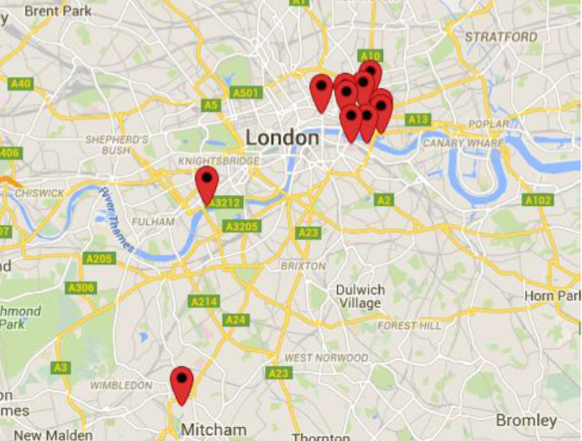
\includegraphics[width=\linewidth]{31-Croucher-figure01}
	\caption{Map of the location of the medieval and post-medieval cemeteries analysed.
		{\normalfont\scriptsize \\ \copyright\ Google Maps
	}}
	\label{fig:31-Croucher-figure01}
\end{figure}

\IJSRAsubsection{Medieval Sites}
The medieval sites used in this research date from the middle- and late-medieval periods, ranging from use between AD 1050-1540, with the middle ages ending with the 1500’s Protestant Reformation.  Of the eight medieval cemeteries excavated and published by the Museum of London, six contained individuals exhibiting interpersonal violence and were included in the study, summing 30 individuals from Merton Priory, Spital Square, East Smithfield Black Death, Guildhall Yard, Bermondsey Abbey and St. Mary Grace cemeteries. These sites included 26 males exhibiting 29 traumas and four females exhibiting four traumas, and are all located in London within a 5 miles radius.  
After the Norman invasion of England in 1066, numerous power struggles for kingship occurred, including the Wars of the Roses and the 100 Years Wars between England and France.  Consequently violence is often deemed a social norm in medieval life, with state war lasting from months to years at a time and waging in recurrent years \parencites{allmand1988}{goodman1990}{turvey2010}.  

The medieval civilisation lacked institutional condemnation of violence in the lower classes, whilst the ruling class of Barons and Earls, utilising large numbers of knights, maintained, gained and annexed land and power through violence. All layers of society maintained a forced connection to war to prove loyalty to those above them in the ‘Great Chain of Being’ and due to the feudal society, tying land owners to landlords and necessitating their supply of men for battle at any needed time \parencite[8]{turvey2010}. 
Thus, aggression has been defined as a reality of medieval lifestyle, used openly across society, and has been likened to modern verbal insults: an unpleasant but socially acceptable normality \parencite{meyerson2004}.

Despite the City of London typically remaining loyal to The Crown at the Tower of London, men were still exploited as soldiers in times of need. With \SI{90}\percent of the population relying on agriculture in the 15th century, 
harvest failure was a further trigger of unrest effecting urban and rural areas alike, alongside the plague of the middle 1300’s, 1420’s, 1430’s and other epidemics throughout the 15th century \parencite{turvey2010}. 
Finally, whilst \textcite{meyerson2004} state most organised violence to have been male orientated, its casual nature is believed to have allowed females to openly participate in violence, and females were often targets of violence in raids and attack. This suggests violence could be prevalent at a high level in both sexes in the medieval sample.

\IJSRAsubsection{Post-medieval} 
The post-medieval sites used in this research date from the 16th to the 19th centuries.  Of the 12 post-medieval cemeteries excavated and published by the Museum of London, five sites included individuals with interpersonal violence and were included in this study, summing 19 individuals from St. Benet Sherehog, St. Brides Lower Cemetery Farringdon, Chelsea Old Church, Broadgate and St. Thomas Hospital cemeteries. These sites included 15 males exhibiting 21 traumas, and four females exhibiting five traumas, and are all located in London within an 11 miles radius.  
  
Historical studies have indicated a decline in violence and homicide rates in the post-medieval period, with analysis possible due to the Elizabethan Assize Courts and improved documentation \parencite{gurr1981}.  
Declining violence correlates with increased jurisdiction and stabilised court policies as time advanced \parencites{samaha1974}{stone1983}{sharpe1985}{cockburn1997}. 
Periodic increases in violence are frequently cited, however, consequence of population booms, the spread of epidemics, including the 1665 Great Plague of London and 1666 Fire of London, and due to the periodic influx of soldiers and seamen from the six wars between 1690 and 1802. The 18th and 19th centuries saw assaults being increasingly reported, resulting in a greater number of violent incidents in the written record, however this increase in documentation may not correlate to an increase in violence, with it more likely just better illuminating violence levels \parencite{gurr1981}.

\IJSRAsection{Results} 
\begin{figure}[!htb]
	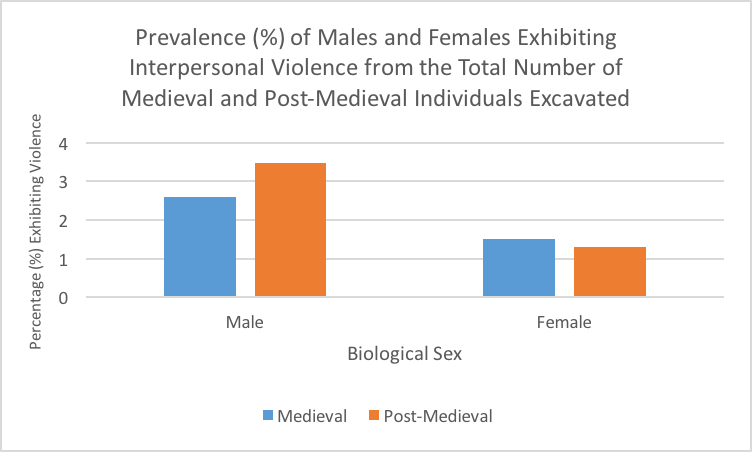
\includegraphics[width=\linewidth]{31-Croucher-figure02}
	\caption{Prevalence of violence within the total number of medieval and post medieval individual excavated in the sites used.
		{\normalfont\scriptsize \\ \copyright\ by \shortauthor
	}}
	\label{fig:31-Croucher-figure02}
\end{figure}
The number of males excavated from all of the cemeteries analysed in the post-medieval period was 58\% less than in the medieval period, as there was a smaller number of cemeteries with individuals exhibiting interpersonal violence in the post-medieval period. By using prevalence, the 58\% decrease in the number of males exhumed is accounted for. 
\Cref{fig:31-Croucher-figure02} shows the prevalence of violence is low in both males and females in the cemeteries excavated, effecting less than 4\% of males and females in both time periods.  The rate of violence against males increased from the medieval to the post-medieval period by 35\%, whilst the rate of violence against females declined by 13.3\%, accounting for the 16\% increase of females exhumed in the post-medieval sample. It was determined that males exhibited 42.3\% more interpersonal violence than females in the medieval period and 62.9\% more than females in the post-medieval period. 

\begin{figure}[!htb]
	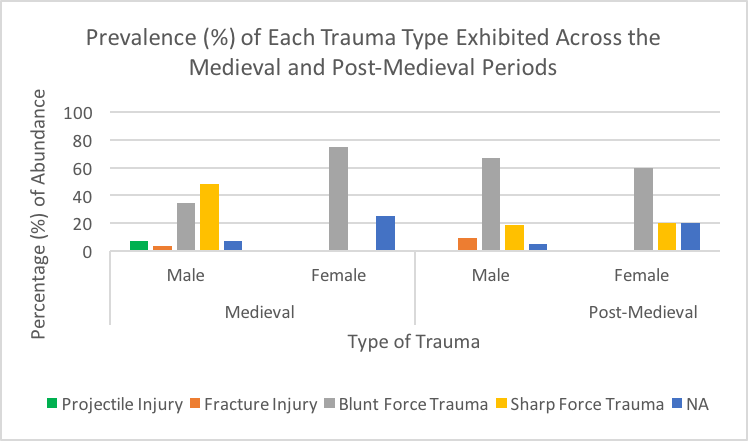
\includegraphics[width=\linewidth]{31-Croucher-figure03}
	\caption{Prevalence of each trauma type exhibited for each biological sex across the medieval and post-medieval periods.
		{\normalfont\scriptsize \\ \copyright\ by \shortauthor
	}}
	\label{fig:31-Croucher-figure03}
\end{figure}
 
Results showed a decline in the range of trauma types from the medieval to the post medieval periods, with the absence of projectile injuries in the post-medieval period \pcref{fig:31-Croucher-figure03}. 
Blunt force trauma remained the dominant trauma type against females across the periods, however the rate dropped in the post-medieval period by 20\%. Female sharp force trauma occurred only in the post-medieval period. Male sharp force trauma declined by 60.6\% in the post-medieval period, whilst blunt force trauma levels increased by 93\% and fracture injuries increased by 179\%. 
 
\begin{figure}[!htb]
	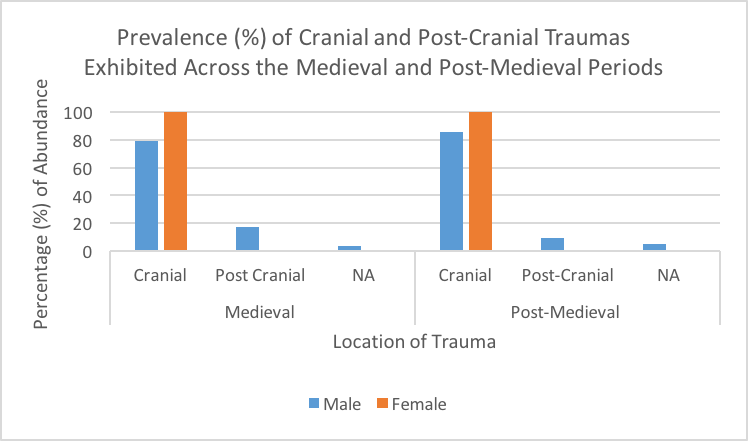
\includegraphics[width=\linewidth]{31-Croucher-figure04}
	\caption{Prevalence of cranial and post cranial traumas for each biological sex across the medieval and post-medieval periods.
		{\normalfont\scriptsize \\ \copyright\ by \shortauthor
	}}
	\label{fig:31-Croucher-figure04}
\end{figure}

The crania remained the dominant location for trauma in both the medieval and post-medieval period for both sexes and females exhibit no post-cranial trauma in either period. The rate of male cranial trauma increased in the post-medieval period by 12\%, whilst post-cranial trauma decreased by 44.8\% \pcref{fig:31-Croucher-figure04}. 
Post-cranial trauma is present in only the male samples, meaning female victims sustained injuries to the face and head only. Post-cranial trauma summed only 14\% of the total number of male injuries across both periods, signifying the body to be an uncommon target in both sexes. 

\begin{figure}[!htb]
	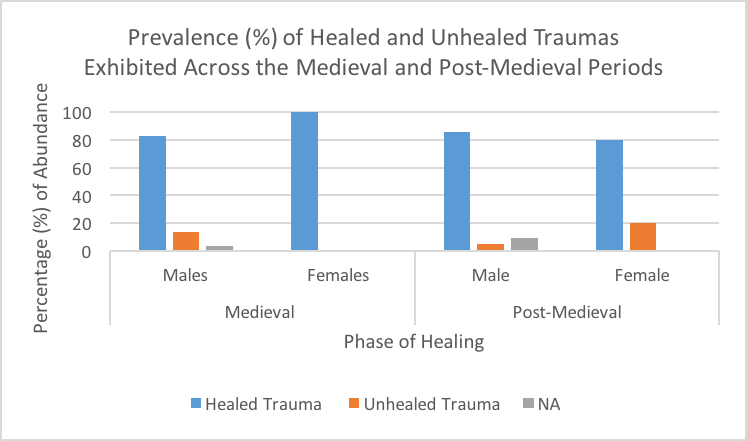
\includegraphics[width=\linewidth]{31-Croucher-figure05}
	\caption{Prevalence of healed and unhealed traumas exhibited, divided by biological sex across the medieval and post-medieval periods.
		{\normalfont\scriptsize \\ \copyright\ by \shortauthor
	}}
	\label{fig:31-Croucher-figure05}
\end{figure}

Healed traumas were the most common trauma types in the sample  \pcref{fig:31-Croucher-figure05}. 
Healed trauma increased in the male sample by 3.6\%, however declined in the female sample by 20\%. Unhealed trauma decreased in the male sample by 64.5\%, and was seen in the female samples only in the post-medieval period. Over both periods, the female sample contained only 11.1\% of unhealed trauma, whilst the males contained 10\%. 

\IJSRAsection{Discussion}%
The larger quantity of violence on male remains across both periods supports prior research, with theories attributing greater male involvement in violence to their more physical lifestyle due to their participation in war and heavy work \parencite{roberts2003}.  

\IJSRAsubsection{Trends of Violence Quantity}
The medieval period has been defined as the peak of violent behaviour in England due to the casual use of violence in lifestyle and the presence of the knightly warrior society, which has been shown to decline uniformly with the rate of violence \parencites{beattie1974}{samaha1974}{hanawalt1976}{given1977}{cockburn1991}. 
Theories explaining this decline have included ‘the civilisation process’ and the rise of the ‘courteous society’ between the 17th to 19th centuries \parencites{beattie1974}{samaha1974}{hanawalt1976}{given1977}{cockburn1991}. 
These models suggest personalities were altered, declining impulsivity, lowering levels of violence and decreasing tolerance towards violence due to the centralisation of authority in the 16th and 17th centuries and the stabilisation of the monarchy \parencite{elias1976}{eisner2001}{eisner2003}. 
No causative correlation, however, can be seen between the rise of the bourgeois society and the fall of violence \parencites{gurr1981}[22]{stone1983}{sharpe1985}.  
The decline in violence against females from the medieval period to the post-medieval period correlates to this trend of lower involvement within violence, however the male results contradict previous research. 

The rise in violence against males can be suggested as a consequence of alterations in economic, social, political, demographic, and personal pressures, leading to heightened emotions and desperation \parencites{gurr1981}{krahn1986}. 
Past peaks of violence include financial crises, war, mass disasters and the spread of epidemics \parencite{stone1983}.  
The decline of English economic stability in the second half of the 1400’s may be accountable for some high levels of violence, resulting in higher levels of agression and uprisings in the late medieval and early post-medieval periods due to instability pressures. However, economic improvements, beginning in the early 15th century, continued into the post-medieval period, removing some financial stress \parencite{saltmarsh1941}. 
The discovered high rate of violence in the London post-medieval sample in this paper could however be consequence of maintained violence levels in the urban environment of London or the growing population’s resulting competitive pressures. The close proximity of the sites and their location in London and close to the River Thames suggests issues of hygiene and the spread of epidemics, including the final Plague of London and the Fire of London, would have majorly impacted the areas \parencite{freestone2012}. 
With stress from a changing environment and resource instability resulting in desperation, the result may have been the observed peak in violence. Furthermore, with numerous religious wars, wars against countries on the continent and civil war, the increase in male violence but decrease in females could be accountable to the different roles of the genders at war time \parencites{gurr1981}{krahn1986}. 

When looking at the number of sites across the medieval and post-medieval period, six of the eight medieval cemeteries analysed by the Museum of London contained individuals exhibiting interpersonal violence, 75\% of the sites, whilst 5 of the 12 post-medieval sites examined included individuals exhibiting violence, 41.7\%. The decline in sites containing individuals exhibiting interpersonal violence can be used to suggest an overall decline in the number of violence cases, or the localisation of violence to specific areas in London.

\IJSRAsubsection{Weapon Type and Social Impacts} 

The absence of projectile injuries in the post-medieval period suggests violence was conducted at this time through close combat fighting using sharp and blunt weaponry, whilst medieval combat included long-distance incidents, seen through the presence of projectile trauma. However, with only two cases, violent methods producing projectile trauma can be deemed uncommon even in the male medieval sample. The results can be used to suggest that specific trauma types were used against the sexes, suggesting social targeting in violence perpetration and boundaries in weapon use, with blunt force trauma the foremost trauma type used against females across both periods and against males in the post-medieval period. The post-medieval period saw blunt force trauma overtaking sharp force trauma as the leading violence cause against males; suggesting fewer stabbings and slicing through the use of blades, sharp tools and glass occurred \parencite{roberts2003}. 
However, the use of specific weapons cannot be conclusively stated as sharp force weaponry can produce blunt force trauma when it is delivered to the skeleton at low velocity, defined as blunt sharp force trauma, potentially overstating the prevalence of blunt force weapons used. 

Documentary evidence suggests medieval weaponry to have predominantly been knives, axes, cudgels and agricultural instruments \parencite{gurr1981}, 
supporting the results in this dissertation due to the predominance of medieval sharp and blunt force traumas. Likewise, documentation from the Elizabethan Assize Courts supports the dominance of blunt and sharp force trauma from the 16th century onwards, stating a dominance of killings through sudden and spontaneous attacks with blunt instruments and knives \parencite{cockburn1997}. 
The court records later stated firearms to account for just 7\% of murders, representing an equally low value of projectile injuries. Indeed, weapon and trauma location can be deemed to be influenced by culture and society, exemplified by the increase of hitting and kicking in the British homicide coroner records coinciding with the rise and broadcasting of modern boxing \parencite{walker1997}. Similarly, U.S. gun trauma outweighs all other harming mechanisms due to the legality and popularity of firearms. 

\IJSRAsubsection{Trauma location} 

The dominance of cranial trauma in the medieval and post-medieval London samples complement wider archaeological violence location research, suggesting the head to be the main target for trauma. The dominance of frontal, parietal and occipital trauma in the sample suggests many of these acts of violence occurred through face-to-face fighting across both time periods \parencite{roberts2003}. 
Cranial injuries are further seen to be dominant in prehistoric research, with high quantities present in Neolithic, Bronze and Iron Age skeletal remains \parencite{berger1995}. 
Equally, the high quantity of cranial and neck traumas exhibited by the 200 Neanderthals analysed from Europe and the Near East suggests violence has consistently centralised around the head and face throughout the past, potentially due to the psychological association of the face and identity \parencite{berger1995}. 

Postcranially, the medieval period contained five post-cranial traumas. Of these, two cases affected the hands, suggesting a defensive stance from the victim, with one case affecting the left hamulus and the second case affecting the right phalanx on the lateral proximal shaft, suggesting the finger was clipped during a defence attempt. The third case was a ‘parry’ fracture to the left radius, suggesting the arms were raised in defence. Indeed, \textcite{roberts2003} state the ribs, scapulae, hands, and forearms to be common areas for defensive wounds, typically to the left hand side due to the dominance of right-handedness.  
The final two cases cannot be labelled as defensive, with both being projectile injuries affecting the left side of the vertebrae.  Differently, in the post-medieval period only two post-cranial traumas were apparent. One of these, a wound on the distal right fibular, was not deemed defensive, whilst the second, a fracture to the left first metocarpophalangeal joint, is potentially the consequence of fist-fighting \parencite{roberts2003}. 
The decline in both multiple injuries and signs of defence could suggest differing styles of fighting, including surprise or organised attacks, however conclusions on fighting styles would require larger data for analysis. 

In relation to sex, the medieval sample contained three males with two injuries, whilst the post-medieval period saw one male and one female with two injuries and one male with six traumas. With only one female exhibiting multiple traumas, extreme violence against females appears uncommon. The medieval and post-medieval cases of multiple traumas were all cranial, suggesting repeated attacks to the body was uncommon in both periods. One case, however, contained six traumas, including five blunt force injuries to the head, affecting the frontal bone and the right side of the crania, with a further injury present on the distal right fibula. This case of multiple trauma is an isolated case within the sample, suggesting extreme and numerous violence was uncommon across both periods.  

Modern trauma provides further comparative data. Of 294 victims of assault from hospital records in the UK in 1986, 43 were females aged 15–46 years, summing 14.6\% of the total number admitted, with males forming 85.4\% \parencite{shepherd1988}.  
Within this sample \textcite{shepherd1988} found facial injuries were the most common location for interpersonal violence trauma, with 88\% of 
females and 84\% of men exhibiting facial bruising \parencite[223]{shepherd1988}. This study suggests facial, qualifying as cranial, trauma remains a dominant trauma form in modern populations across both sexes, complementing the results from the medieval and post-medieval samples. 

\IJSRAsubsection{Phase of healing of the trauma}

The dominance of healed trauma suggests most interpersonal violence related traumas were not the cause, linked to, or received at the same time as death \parencites{lovell1997}{roberts2003}. The dominance of ante-mortem injuries across both periods proposes society did not advocate lethal violence, however smaller brawls and fights were common.

The decrease in peri-mortem trauma in males across the periods could suggest that as violence against males increased in quantity it became less lethal, with casual violence becoming a social norm and potentially resulting in a decline in lethal intent due to its unpremeditated form. The opposite is seen in the female sample, with peri-mortem trauma increasing in correlation with lowering levels of female violence.  This can be used to suggest that as social acceptability of casual violence against females decreased, arguments concerning females became less violently-orientated, as fewer healed traumas were observed. However, the increase in unhealed traumas could suggest that when violence occurred it was more likely to result in lethal violence, explaining the decrease in normative ante-mortem traumas and rise in peri-mortem injuries.

\IJSRAsection{Conclusions}

Considering multiple aspects within the cause and manifestation of the traumas analysed in this study, the research has confirmed the medieval and post-medieval London sample followed normative violence trends in relation to ‘gender’, with males consistently receiving a higher rate of violence than females. The evaluation of the phase of healing of traumas has outlined the rarity of homicide in relation to everyday ‘social’ violence, and highlighted non-lethal violence to be more common. Despite the lack of conclusive reasoning, the rise in violence against males has been suggested to be due to increased social pressures, war and medical desperation, whilst the decrease in female victimisation correlates to wider research on declining violence rates. Further research is necessary to establish why the rate of violence against males increased in the post-medieval period. Finally, the dominance of blunt and sharp force and cranial trauma underpins external research, with head and facial trauma visible in high quantities in studies across all time periods, and as blunt and sharp weaponry is widely stated as the most frequently used weapons in the medieval and post-medieval periods.  


\IJSRAclosing%<---- don’t change this!